\begin{SCn}

\scnsectionheader{\currentname}
\scntext{эпиграф}{Если вещи будут именоваться неправильно, слова потеряют силу и ни одно дело нельзя будет довести до конца. Конфуций 5-6 вв. до н.э.}
\scntext{эпиграф}{Удачно выбранный термин – путь к пониманию и признанию, а неудачно выбранный – путь к забвению.}

\scnstartsubstruct

\scnheader{Предметная область внешних идентификаторов sc-элементов}
\scniselement{предметная область}
\scnsdmainclasssingle{идентификатор}
\scnsdclass{строковый идентификатор;нестроковый идентификатор;атомарный идентификатор;неатомарный идентификатор;идентификатор-контур;идентификатор-файл;идентификатор-множество;идентификатор-кортеж;идентификатор-операция;системный идентификатор}
\scnsdrelation{идентификатор*;основной идентификатор*;системный идентификатор*;последовательность внешних идентификаторов*}

\scnheader{идентификатор}
\scnidtf{sc-знак внешнего идентификатора некоторого sc-элемента}
\scnidtf{внешний идентификатор sc-элемента}
\scnidtf{sc-знак sc-идентификатора}
\scnrelto{второй домен}{идентификатор}
\scnsubset{файл}
\scnexplanation{Под \textbf{\textit{идентификатором}} понимается файл, который может быть использован для обозначения (именования) той или иной сущности в рамках какого-либо \textit{внешнего языка}. \textbf{\textit{Идентификатором}} может быть, в том числе, \textit{изображение}.

Существенно подчеркнуть, что выбор \textit{идентификаторов} влияет только на первичное восприятие принимаемых сообщений и на конечный этап синтеза передаваемых сообщений, но никак не влияет на рассуждения.

Другими словами, \textbf{\textit{идентификатор}} это \textit{sc-знак файла}, в котором хранится в определенном формате электронный образ одного из экземпляров класса синтаксически эквивалентных конструкций, все или многие из которых, входя во внешние тексты, обозначают ту же сущность, что и соответствующий им \textit{sc-элемент}.}
\scnreltoset{разбиение}{строковый идентификатор;нестроковый идентификатор}

\scnheader{строковый идентификатор}
\scnexplanation{Наиболее часто используемыми \textit{идентификаторами} являются \textbf{\textit{строковые идентификаторы}}, которые представляют собой строку символов какого-либо фиксированного алфавита.}
\scnreltoset{разбиение}{атомарный идентификатор;неатомарный идентификатор}

\scnheader{нестроковый идентификатор}
\scntext{примечание}{Помимо \textit{строковых идентификаторов}, выделяются \textbf{\textit{нестроковые идентификаторы}}, которые идентифицируют объекты при помощи графических иллюстраций, символов, иероглифов, пиктограмм и др.}

\scnheader{атомарный идентификатор}
\scntext{примечание}{\textbf{\textit{атомарный идентификатор}} - это \textit{идентификатор}, при формировании которого не используются другие \textit{идентификаторы}.}
\scnhaselementrole{пример}{\textnormal{[треугольник]}}

\scnheader{неатомарный идентификатор}
\scntext{примечание}{\textbf{\textit{неатомарный идентификатор}} - это \textit{идентификатор}, в состав которого входят другие \textit{идентификаторы}.}
\scnhaselementrole{пример}{
\textnormal{[Треугк.(Тчк.А; Тчк.B; Тчк.С)]}\\
\scntext{комментарий}{Приведен пример \textit{неатомарного идентификатора} - \textit{идентификатор} треугольника АВС. В своем составе данный \textit{идентификатор} содержит \textit{атомарные идентификаторы} трех точек, задающих этот треугольник: точка А, точка B и точка C.}}
\scnsuperset{идентификатор-контур}
\scnsuperset{идентификатор-ссылка}
\scnsuperset{идентификатор-множество}
\scnsuperset{идентификатор-кортеж}
\scnsuperset{идентификатор-операция}

\scnheader{идентификатор-контур}
\scnidtf{[* *]-идентификатор}
\scnexplanation{\textbf{\textit{идентификатор-контур}} - \textit{идентификатор sc-элемента}, который обозначает семантически эквивалентную \textit{структуру} для текста в скобках со звездочками, записанного на некотором внешнем языке, т.е. результат трансляции текста в скобках в \textit{SC-код}.}

\scnheader{идентификатор-файл}
\scnidtf{[ ]-идентификатор}
\scnidtf{идентификатор-рамка}
\scnexplanation{\textbf{\textit{идентификатор-файл}} представляет собой \textit{идентификатор sc-элемента}, который является \textit{файлом}, содержимым которого является некоторый текст в квадратных скобках, записанный на каком-либо \textit{внешнем языке}.}

\scnheader{идентификатор-множество}
\scnidtf{\{ \}-идентификатор}
\scnexplanation{\textbf{\textit{идентификатор-множество}} представляет собой \textit{идентификатор sc-элемента}, являющегося \textit{множеством}, которому принадлежат элементы, \textit{идентификаторы} которых перечисляются в фигурных скобках через знак точки с запятой «;».

В скобках должны быть перечислены все элементы идентифицируемого \textit{множества}. Если перечисляются не все элементы идентифицированного \textit{множества}, то после последнего элемента ставится знак «;», а далее ставится знак «…».}
\scnrelfrom{описание типичного экземпляра}{
\scnfilelong{
\begin{figure}[H]
\centering
\begin{subfigure}
  \centering
  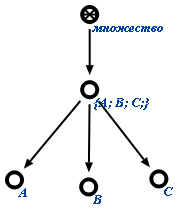
\includegraphics[width=0.3\linewidth]{figures/sd_identifiers/typical_sc_neighborhood_for_sc_identifier_set1.png}
  \label{fig:sub1}
\end{subfigure}
\begin{subfigure}
  \centering
  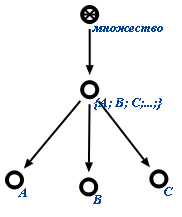
\includegraphics[width=0.3\linewidth]{figures/sd_identifiers/typical_sc_neighborhood_for_sc_identifier_set2.png}
  \label{fig:sub2}
\end{subfigure}
\end{figure}
}}

\scnheader{идентификатор-кортеж}
\scnidtf{< >-идентификатор}
\scnexplanation{\textbf{\textit{идентификатор-кортеж}} – это \textit{идентификатор ориентированного множества}, которому принадлежат элементы, идентификаторы которых перечислены в скобках через знак точки с запятой «;». При этом считается, что всем элементам описываемого \textit{множества} приписаны \textit{числовые атрибуты}, соответствующие порядку следования имени элемента в перечислении.}
\scnrelfrom{описание типичного экземпляра}{
\scnfilelong{
\begin{figure}[H]
\centering
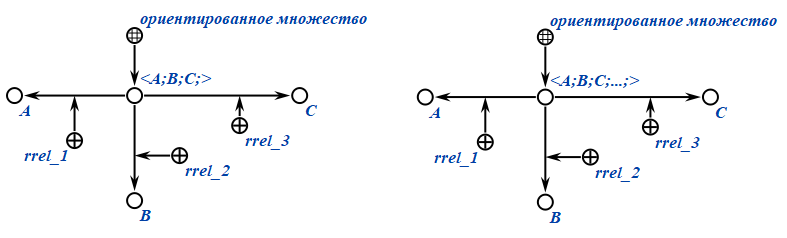
\includegraphics[width=1\linewidth]{figures/sd_identifiers/typical_sc_neighborhood_for_sc_identifier_tuple_set.png}
\end{figure}
}}

\scnheader{идентификатор-операция}
\scnidtf{(+)-идентификатор}
\scnexplanation{\textbf{\textit{идентификатор-операция}} – это \textit{идентификатор sc-элемента}, являющегося результатом \textit{арифметической}, теоретико-множественной или \textit{логической операции}, обозначение которой записано какими-либо специальными символами в круглых скобках.}
\scnrelfrom{описание типичного экземпляра}{
\scnfilelong{
\begin{figure}[H]
\centering
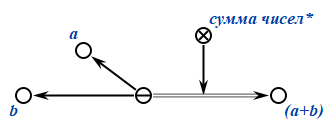
\includegraphics[width=0.5\linewidth]{figures/sd_identifiers/typical_sc_neighborhood_for_sc_identifier_operation_set.png}
\end{figure}
}}

\scnheader{идентификатор*}
\scniselement{бинарное отношение}
\scniselement{ориентированное отношение}
\scnexplanation{\textbf{\textit{идентификатор*}}- это бинарное \textit{ориентированное отношение}, связывающее \textit{sc-элемент} с \textit{файлом}, содержащим его идентификатор на каком-либо \textit{внешнем языке}.}

\scnheader{основной идентификатор*}
\scnsubset{идентификатор*}
\scnexplanation{\textbf{\textit{основной идентификатор*}}- это бинарное \textit{ориентированное отношение}, связывающее sc-элемент с \textit{файлом}, содержащим его основной идентификатор, т.е. \textit{идентификатор}, который должен быть уникален в рамках одного \textit{внешнего языка}.}

\scnheader{системный идентификатор*}
\scnsubset{идентификатор*}
\scnexplanation{\textbf{\textit{системный идентификатор*}}- это бинарное \textit{ориентированное отношение}, связывающее \textit{sc-элемент} с \textit{файлом}, содержащим его \textit{системный идентификатор}.}

\scnheader{системный идентификатор}
\scnidtf{глобальный идентификатор}
\scnsubset{идентификатор}
\scnrelto{второй домен}{системный идентификатор}
\scnexplanation{\textbf{\textit{системный идентификатор}} - это \textit{идентификатор}, являющийся уникальным в рамках всей \textit{базы знаний}. Данный \textit{идентификатор}, как правило, используется в исходных текстах базы знаний нижнего уровня. Для обеспечения интернационализации рекомендуется записывать \textbf{\textit{системные идентификаторы}} на английском языке.

Символами, использующимися в \textbf{\textit{системном идентификаторе}}, могут быть буквы латинского алфавита, цифры, знак нижнего подчеркивания и знак тире. 

Таким образом, наиболее целесообразно формировать \textbf{\textit{системный идентификатор}} \textit{sc-элемента} из основного англоязычного путем замены всех символов, не входящих в описанный выше алфавит на символ «\_».

Например:\\
основной англоязычный идентификатор: Partition. SCs-code. Dividers\\
\textbf{\textit{системный идентификатор}}: Partition\_SCs-code\_Dividers\\
Для именования \textit{sc-элементов}, являющихся знаками \textit{ролевых отношений}, вместо знака «’» в \textbf{\textit{системном идентификаторе}} используется приставка «rrel» и далее после нижнего подчеркивания записывается имя \textit{ролевого отношения}.\\
Для именования \textit{sc-элементов}, являющихся знаками \textit{неролевых отношений}, вместо знака «*» в \textit{системном идентификаторе} используется приставка «nrel» и далее после нижнего подчеркивания записывается имя \textit{неролевого отношения}.\\
Для именования \textit{sc-элементов}, являющихся знаками \textit{классов} понятий в идентификаторе используется приставка «concept» и далее после нижнего подчеркивания записывается имя \textit{класса}.\\
Для именования \textit{sc-элементов}, являющихся знаками \textit{структур} в идентификаторе используется приставка «struct» и далее после нижнего подчеркивания записывается имя \textit{структуры}.\\
Для именования \textit{sc-элементов}, являющихся знаками \textit{кортежей} в идентификаторе используется приставка «tuple» и далее после нижнего подчеркивания записывается имя \textit{кортежа}.

Например:\\
rrel\_summand\\
/*ролевое отношение «слагаемое’»*/\\
nrel\_inclusion\\
/*неролевое отношение «включение*»*/\\
concept\_triangle\\
/*класс «треугольник»*/\\
struct\_Triangle\_A\_B\_C\\
/*структура «Треугк(ТчкA;ТчкB;ТчкC)»*/
}

\scnheader{последовательность внешних идентификаторов*}
\scniselement{отношение строгого порядка}
\scnexplanation{\textbf{\textit{последовательность внешних идентификаторов*}} - это бинарное \textit{ориентированное отношение}, связывающее между собой связки отношения \textit{идентификатор*}, имеющие общий первый компонент, и упорядочивающее таким образом идентификаторы одного объекта между собой по некоторому критерию. Чаще всего таким критерием является степень ассоциируемости того или иного идентификатора с описываемым понятием, его «узнаваемость», «точность» и т.д.}

\scnendstruct

\end{SCn}